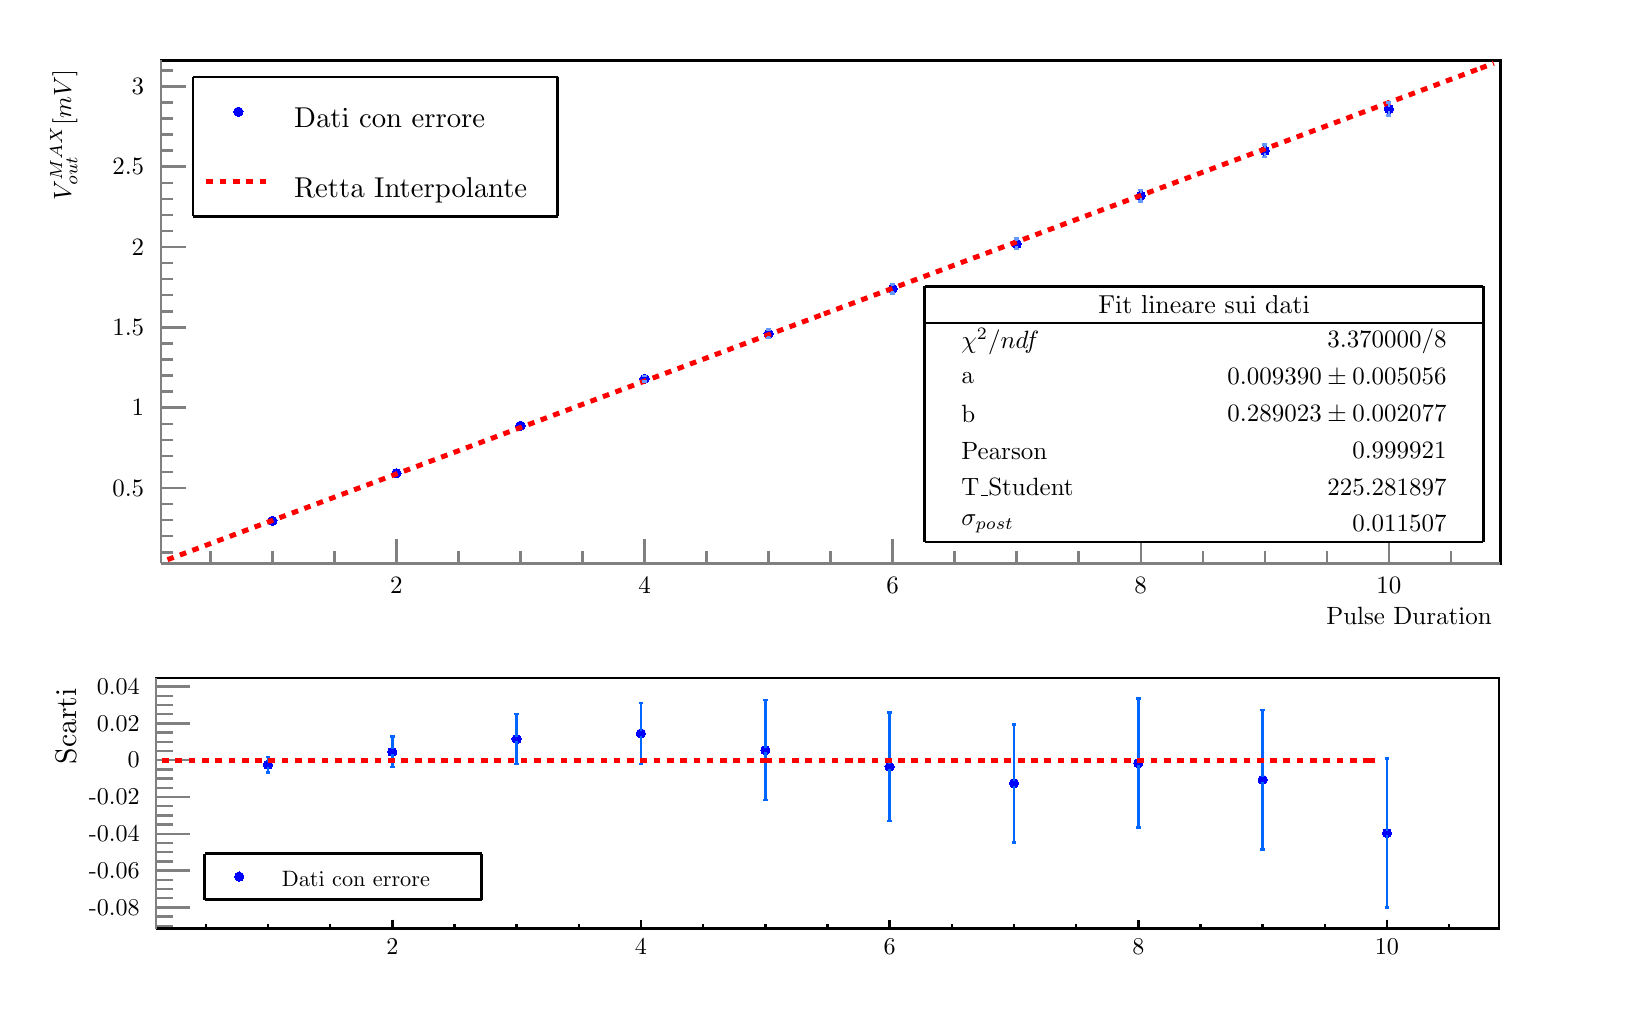
\begin{tikzpicture}
\pgfdeclareplotmark{cross} {
\pgfpathmoveto{\pgfpoint{-0.3\pgfplotmarksize}{\pgfplotmarksize}}
\pgfpathlineto{\pgfpoint{+0.3\pgfplotmarksize}{\pgfplotmarksize}}
\pgfpathlineto{\pgfpoint{+0.3\pgfplotmarksize}{0.3\pgfplotmarksize}}
\pgfpathlineto{\pgfpoint{+1\pgfplotmarksize}{0.3\pgfplotmarksize}}
\pgfpathlineto{\pgfpoint{+1\pgfplotmarksize}{-0.3\pgfplotmarksize}}
\pgfpathlineto{\pgfpoint{+0.3\pgfplotmarksize}{-0.3\pgfplotmarksize}}
\pgfpathlineto{\pgfpoint{+0.3\pgfplotmarksize}{-1.\pgfplotmarksize}}
\pgfpathlineto{\pgfpoint{-0.3\pgfplotmarksize}{-1.\pgfplotmarksize}}
\pgfpathlineto{\pgfpoint{-0.3\pgfplotmarksize}{-0.3\pgfplotmarksize}}
\pgfpathlineto{\pgfpoint{-1.\pgfplotmarksize}{-0.3\pgfplotmarksize}}
\pgfpathlineto{\pgfpoint{-1.\pgfplotmarksize}{0.3\pgfplotmarksize}}
\pgfpathlineto{\pgfpoint{-0.3\pgfplotmarksize}{0.3\pgfplotmarksize}}
\pgfpathclose
\pgfusepathqstroke
}
\pgfdeclareplotmark{cross*} {
\pgfpathmoveto{\pgfpoint{-0.3\pgfplotmarksize}{\pgfplotmarksize}}
\pgfpathlineto{\pgfpoint{+0.3\pgfplotmarksize}{\pgfplotmarksize}}
\pgfpathlineto{\pgfpoint{+0.3\pgfplotmarksize}{0.3\pgfplotmarksize}}
\pgfpathlineto{\pgfpoint{+1\pgfplotmarksize}{0.3\pgfplotmarksize}}
\pgfpathlineto{\pgfpoint{+1\pgfplotmarksize}{-0.3\pgfplotmarksize}}
\pgfpathlineto{\pgfpoint{+0.3\pgfplotmarksize}{-0.3\pgfplotmarksize}}
\pgfpathlineto{\pgfpoint{+0.3\pgfplotmarksize}{-1.\pgfplotmarksize}}
\pgfpathlineto{\pgfpoint{-0.3\pgfplotmarksize}{-1.\pgfplotmarksize}}
\pgfpathlineto{\pgfpoint{-0.3\pgfplotmarksize}{-0.3\pgfplotmarksize}}
\pgfpathlineto{\pgfpoint{-1.\pgfplotmarksize}{-0.3\pgfplotmarksize}}
\pgfpathlineto{\pgfpoint{-1.\pgfplotmarksize}{0.3\pgfplotmarksize}}
\pgfpathlineto{\pgfpoint{-0.3\pgfplotmarksize}{0.3\pgfplotmarksize}}
\pgfpathclose
\pgfusepathqfillstroke
}
\pgfdeclareplotmark{newstar} {
\pgfpathmoveto{\pgfqpoint{0pt}{\pgfplotmarksize}}
\pgfpathlineto{\pgfqpointpolar{44}{0.5\pgfplotmarksize}}
\pgfpathlineto{\pgfqpointpolar{18}{\pgfplotmarksize}}
\pgfpathlineto{\pgfqpointpolar{-20}{0.5\pgfplotmarksize}}
\pgfpathlineto{\pgfqpointpolar{-54}{\pgfplotmarksize}}
\pgfpathlineto{\pgfqpointpolar{-90}{0.5\pgfplotmarksize}}
\pgfpathlineto{\pgfqpointpolar{234}{\pgfplotmarksize}}
\pgfpathlineto{\pgfqpointpolar{198}{0.5\pgfplotmarksize}}
\pgfpathlineto{\pgfqpointpolar{162}{\pgfplotmarksize}}
\pgfpathlineto{\pgfqpointpolar{134}{0.5\pgfplotmarksize}}
\pgfpathclose
\pgfusepathqstroke
}
\pgfdeclareplotmark{newstar*} {
\pgfpathmoveto{\pgfqpoint{0pt}{\pgfplotmarksize}}
\pgfpathlineto{\pgfqpointpolar{44}{0.5\pgfplotmarksize}}
\pgfpathlineto{\pgfqpointpolar{18}{\pgfplotmarksize}}
\pgfpathlineto{\pgfqpointpolar{-20}{0.5\pgfplotmarksize}}
\pgfpathlineto{\pgfqpointpolar{-54}{\pgfplotmarksize}}
\pgfpathlineto{\pgfqpointpolar{-90}{0.5\pgfplotmarksize}}
\pgfpathlineto{\pgfqpointpolar{234}{\pgfplotmarksize}}
\pgfpathlineto{\pgfqpointpolar{198}{0.5\pgfplotmarksize}}
\pgfpathlineto{\pgfqpointpolar{162}{\pgfplotmarksize}}
\pgfpathlineto{\pgfqpointpolar{134}{0.5\pgfplotmarksize}}
\pgfpathclose
\pgfusepathqfillstroke
}
\definecolor{c}{rgb}{1,1,1};
\draw [color=c, fill=c] (0,0) rectangle (20,12.406);
\draw [color=c, fill=c] (0.1,0.24812) rectangle (19.8,12.0338);
\draw [color=c, fill=c] (1.68337,5.60968) rectangle (18.6974,11.9961);
\definecolor{c}{rgb}{0,0,0};
\draw [c,line width=0.9] (1.68337,5.60968) -- (1.68337,11.9961) -- (18.6974,11.9961) -- (18.6974,5.60968) -- (1.68337,5.60968);
\definecolor{c}{rgb}{1,1,1};
\draw [color=c, fill=c] (1.68337,5.60968) rectangle (18.6974,11.9961);
\definecolor{c}{rgb}{0,0,0};
\draw [c,line width=0.9] (1.68337,5.60968) -- (1.68337,11.9961) -- (18.6974,11.9961) -- (18.6974,5.60968) -- (1.68337,5.60968);
\definecolor{c}{rgb}{0.5,0.5,0.5};
\draw [c,line width=0.9] (1.68337,5.60968) -- (18.6974,5.60968);
\draw [c,line width=0.9] (4.67658,5.91504) -- (4.67658,5.60968);
\draw [c,line width=0.9] (5.46426,5.76236) -- (5.46426,5.60968);
\draw [c,line width=0.9] (6.25195,5.76236) -- (6.25195,5.60968);
\draw [c,line width=0.9] (7.03963,5.76236) -- (7.03963,5.60968);
\draw [c,line width=0.9] (7.82732,5.91504) -- (7.82732,5.60968);
\draw [c,line width=0.9] (8.61501,5.76236) -- (8.61501,5.60968);
\draw [c,line width=0.9] (9.40269,5.76236) -- (9.40269,5.60968);
\draw [c,line width=0.9] (10.1904,5.76236) -- (10.1904,5.60968);
\draw [c,line width=0.9] (10.9781,5.91504) -- (10.9781,5.60968);
\draw [c,line width=0.9] (11.7658,5.76236) -- (11.7658,5.60968);
\draw [c,line width=0.9] (12.5534,5.76236) -- (12.5534,5.60968);
\draw [c,line width=0.9] (13.3411,5.76236) -- (13.3411,5.60968);
\draw [c,line width=0.9] (14.1288,5.91504) -- (14.1288,5.60968);
\draw [c,line width=0.9] (14.9165,5.76236) -- (14.9165,5.60968);
\draw [c,line width=0.9] (15.7042,5.76236) -- (15.7042,5.60968);
\draw [c,line width=0.9] (16.4919,5.76236) -- (16.4919,5.60968);
\draw [c,line width=0.9] (17.2796,5.91504) -- (17.2796,5.60968);
\draw [c,line width=0.9] (4.67658,5.91504) -- (4.67658,5.60968);
\draw [c,line width=0.9] (3.88889,5.76236) -- (3.88889,5.60968);
\draw [c,line width=0.9] (3.1012,5.76236) -- (3.1012,5.60968);
\draw [c,line width=0.9] (2.31352,5.76236) -- (2.31352,5.60968);
\draw [c,line width=0.9] (17.2796,5.91504) -- (17.2796,5.60968);
\draw [c,line width=0.9] (18.0672,5.76236) -- (18.0672,5.60968);
\definecolor{c}{rgb}{0,0,0};
\draw [anchor=base] (4.67658,5.22075) node[scale=0.902611, color=c, rotate=0]{2};
\draw [anchor=base] (7.82732,5.22075) node[scale=0.902611, color=c, rotate=0]{4};
\draw [anchor=base] (10.9781,5.22075) node[scale=0.902611, color=c, rotate=0]{6};
\draw [anchor=base] (14.1288,5.22075) node[scale=0.902611, color=c, rotate=0]{8};
\draw [anchor=base] (17.2796,5.22075) node[scale=0.902611, color=c, rotate=0]{10};
\draw [anchor= east] (18.6974,4.94968) node[scale=0.902611, color=c, rotate=0]{Pulse Duration};
\definecolor{c}{rgb}{0.5,0.5,0.5};
\draw [c,line width=0.9] (1.68337,5.60968) -- (1.68337,11.9961);
\draw [c,line width=0.9] (2.00362,6.56654) -- (1.68337,6.56654);
\draw [c,line width=0.9] (1.84349,6.77055) -- (1.68337,6.77055);
\draw [c,line width=0.9] (1.84349,6.97456) -- (1.68337,6.97456);
\draw [c,line width=0.9] (1.84349,7.17857) -- (1.68337,7.17857);
\draw [c,line width=0.9] (1.84349,7.38258) -- (1.68337,7.38258);
\draw [c,line width=0.9] (2.00362,7.58659) -- (1.68337,7.58659);
\draw [c,line width=0.9] (1.84349,7.7906) -- (1.68337,7.7906);
\draw [c,line width=0.9] (1.84349,7.99461) -- (1.68337,7.99461);
\draw [c,line width=0.9] (1.84349,8.19862) -- (1.68337,8.19862);
\draw [c,line width=0.9] (1.84349,8.40263) -- (1.68337,8.40263);
\draw [c,line width=0.9] (2.00362,8.60664) -- (1.68337,8.60664);
\draw [c,line width=0.9] (1.84349,8.81065) -- (1.68337,8.81065);
\draw [c,line width=0.9] (1.84349,9.01466) -- (1.68337,9.01466);
\draw [c,line width=0.9] (1.84349,9.21867) -- (1.68337,9.21867);
\draw [c,line width=0.9] (1.84349,9.42268) -- (1.68337,9.42268);
\draw [c,line width=0.9] (2.00362,9.62669) -- (1.68337,9.62669);
\draw [c,line width=0.9] (1.84349,9.8307) -- (1.68337,9.8307);
\draw [c,line width=0.9] (1.84349,10.0347) -- (1.68337,10.0347);
\draw [c,line width=0.9] (1.84349,10.2387) -- (1.68337,10.2387);
\draw [c,line width=0.9] (1.84349,10.4427) -- (1.68337,10.4427);
\draw [c,line width=0.9] (2.00362,10.6467) -- (1.68337,10.6467);
\draw [c,line width=0.9] (1.84349,10.8507) -- (1.68337,10.8507);
\draw [c,line width=0.9] (1.84349,11.0548) -- (1.68337,11.0548);
\draw [c,line width=0.9] (1.84349,11.2588) -- (1.68337,11.2588);
\draw [c,line width=0.9] (1.84349,11.4628) -- (1.68337,11.4628);
\draw [c,line width=0.9] (2.00362,11.6668) -- (1.68337,11.6668);
\draw [c,line width=0.9] (2.00362,6.56654) -- (1.68337,6.56654);
\draw [c,line width=0.9] (1.84349,6.36253) -- (1.68337,6.36253);
\draw [c,line width=0.9] (1.84349,6.15852) -- (1.68337,6.15852);
\draw [c,line width=0.9] (1.84349,5.95452) -- (1.68337,5.95452);
\draw [c,line width=0.9] (1.84349,5.75051) -- (1.68337,5.75051);
\draw [c,line width=0.9] (2.00362,11.6668) -- (1.68337,11.6668);
\draw [c,line width=0.9] (1.84349,11.8708) -- (1.68337,11.8708);
\definecolor{c}{rgb}{0,0,0};
\draw [anchor= east] (1.58487,6.56654) node[scale=0.902611, color=c, rotate=0]{0.5};
\draw [anchor= east] (1.58487,7.58659) node[scale=0.902611, color=c, rotate=0]{1};
\draw [anchor= east] (1.58487,8.60664) node[scale=0.902611, color=c, rotate=0]{1.5};
\draw [anchor= east] (1.58487,9.62669) node[scale=0.902611, color=c, rotate=0]{2};
\draw [anchor= east] (1.58487,10.6467) node[scale=0.902611, color=c, rotate=0]{2.5};
\draw [anchor= east] (1.58487,11.6668) node[scale=0.902611, color=c, rotate=0]{3};
\draw [anchor= east] (0.452513,11.9961) node[scale=0.902611, color=c, rotate=90]{$V_{out}^{MAX} [mV]$};
\definecolor{c}{rgb}{0,0,1};
\foreach \P in {(3.1012,6.15036), (4.67658,6.75423), (6.25195,7.3581), (7.82732,7.95381), (9.40269,8.52504), (10.9781,9.09626), (12.5534,9.66749), (14.1288,10.2795), (15.7042,10.8507), (17.2796,11.3812)}{\draw[mark options={color=c,fill=c},mark
 size=1.681682pt, line width=0.000000pt, mark=*] plot coordinates {\P};}
\definecolor{c}{rgb}{1,0,0};
\draw [c,dash pattern=on 2.40pt off 2.40pt ,line width=1.8] (1.76844,5.65646) -- (1.93858,5.72014) -- (2.10872,5.78382) -- (2.27886,5.8475) -- (2.449,5.91118) -- (2.61914,5.97486) -- (2.78928,6.03854) -- (2.95942,6.10222) -- (3.12956,6.1659) --
 (3.2997,6.22958) -- (3.46984,6.29326) -- (3.63998,6.35694) -- (3.81012,6.42062) -- (3.98026,6.4843) -- (4.1504,6.54798) -- (4.32054,6.61166) -- (4.49068,6.67534) -- (4.66082,6.73903) -- (4.83096,6.80271) -- (5.0011,6.86639) -- (5.17124,6.93007) --
 (5.34138,6.99375) -- (5.51152,7.05743) -- (5.68166,7.12111) -- (5.8518,7.18479) -- (6.02194,7.24847) -- (6.19208,7.31215) -- (6.36222,7.37583) -- (6.53236,7.43951) -- (6.70251,7.50319) -- (6.87265,7.56687) -- (7.04279,7.63055) -- (7.21293,7.69423)
 -- (7.38307,7.75791) -- (7.55321,7.82159) -- (7.72335,7.88527) -- (7.89349,7.94896) -- (8.06363,8.01264) -- (8.23377,8.07632) -- (8.40391,8.14) -- (8.57405,8.20368) -- (8.74419,8.26736) -- (8.91433,8.33104) -- (9.08447,8.39472) -- (9.25461,8.4584)
 -- (9.42475,8.52208) -- (9.59489,8.58576) -- (9.76503,8.64944) -- (9.93517,8.71312) -- (10.1053,8.7768);
\draw [c,dash pattern=on 2.40pt off 2.40pt ,line width=1.8] (10.1053,8.7768) -- (10.2755,8.84048) -- (10.4456,8.90416) -- (10.6157,8.96784) -- (10.7859,9.03152) -- (10.956,9.0952) -- (11.1262,9.15888) -- (11.2963,9.22256) -- (11.4664,9.28625) --
 (11.6366,9.34993) -- (11.8067,9.41361) -- (11.9769,9.47729) -- (12.147,9.54097) -- (12.3171,9.60465) -- (12.4873,9.66833) -- (12.6574,9.73201) -- (12.8276,9.79569) -- (12.9977,9.85937) -- (13.1678,9.92305) -- (13.338,9.98673) -- (13.5081,10.0504) --
 (13.6783,10.1141) -- (13.8484,10.1778) -- (14.0185,10.2415) -- (14.1887,10.3051) -- (14.3588,10.3688) -- (14.529,10.4325) -- (14.6991,10.4962) -- (14.8692,10.5599) -- (15.0394,10.6235) -- (15.2095,10.6872) -- (15.3797,10.7509) -- (15.5498,10.8146)
 -- (15.7199,10.8783) -- (15.8901,10.9419) -- (16.0602,11.0056) -- (16.2304,11.0693) -- (16.4005,11.133) -- (16.5706,11.1967) -- (16.7408,11.2603) -- (16.9109,11.324) -- (17.0811,11.3877) -- (17.2512,11.4514) -- (17.4213,11.5151) -- (17.5915,11.5787)
 -- (17.7616,11.6424) -- (17.9318,11.7061) -- (18.1019,11.7698) -- (18.272,11.8335) -- (18.4422,11.8971);
\draw [c,dash pattern=on 2.40pt off 2.40pt ,line width=1.8] (18.4422,11.8971) -- (18.6123,11.9608);
\definecolor{c}{rgb}{0.4,0.6,1};
\draw [c,line width=0.9] (7.82732,7.98388) -- (7.82732,7.98767);
\draw [c,line width=0.9] (7.79725,7.98767) -- (7.8574,7.98767);
\draw [c,line width=0.9] (7.82732,7.92373) -- (7.82732,7.91995);
\draw [c,line width=0.9] (7.79725,7.91995) -- (7.8574,7.91995);
\draw [c,line width=0.9] (9.40269,8.55511) -- (9.40269,8.5804);
\draw [c,line width=0.9] (9.37262,8.5804) -- (9.43277,8.5804);
\draw [c,line width=0.9] (9.40269,8.49496) -- (9.40269,8.46967);
\draw [c,line width=0.9] (9.37262,8.46967) -- (9.43277,8.46967);
\draw [c,line width=0.9] (10.9781,9.12634) -- (10.9781,9.15646);
\draw [c,line width=0.9] (10.948,9.15646) -- (11.0081,9.15646);
\draw [c,line width=0.9] (10.9781,9.06619) -- (10.9781,9.03606);
\draw [c,line width=0.9] (10.948,9.03606) -- (11.0081,9.03606);
\draw [c,line width=0.9] (12.5534,9.69756) -- (12.5534,9.73292);
\draw [c,line width=0.9] (12.5234,9.73292) -- (12.5835,9.73292);
\draw [c,line width=0.9] (12.5534,9.63741) -- (12.5534,9.60206);
\draw [c,line width=0.9] (12.5234,9.60206) -- (12.5835,9.60206);
\draw [c,line width=0.9] (14.1288,10.3096) -- (14.1288,10.3509);
\draw [c,line width=0.9] (14.0987,10.3509) -- (14.1589,10.3509);
\draw [c,line width=0.9] (14.1288,10.2494) -- (14.1288,10.2081);
\draw [c,line width=0.9] (14.0987,10.2081) -- (14.1589,10.2081);
\draw [c,line width=0.9] (15.7042,10.8808) -- (15.7042,10.9279);
\draw [c,line width=0.9] (15.6741,10.9279) -- (15.7343,10.9279);
\draw [c,line width=0.9] (15.7042,10.8207) -- (15.7042,10.7736);
\draw [c,line width=0.9] (15.6741,10.7736) -- (15.7343,10.7736);
\draw [c,line width=0.9] (17.2796,11.4112) -- (17.2796,11.4639);
\draw [c,line width=0.9] (17.2495,11.4639) -- (17.3096,11.4639);
\draw [c,line width=0.9] (17.2796,11.3511) -- (17.2796,11.2985);
\draw [c,line width=0.9] (17.2495,11.2985) -- (17.3096,11.2985);
\definecolor{c}{rgb}{1,1,1};
\draw [color=c, fill=c] (11.3835,5.8797) rectangle (18.4812,9.12782);
\definecolor{c}{rgb}{0,0,0};
\draw [c,line width=0.9] (11.3835,5.8797) -- (18.4812,5.8797);
\draw [c,line width=0.9] (18.4812,5.8797) -- (18.4812,9.12782);
\draw [c,line width=0.9] (18.4812,9.12782) -- (11.3835,9.12782);
\draw [c,line width=0.9] (11.3835,9.12782) -- (11.3835,5.8797);
\draw (14.9323,8.89581) node[scale=0.936041, color=c, rotate=0]{Fit lineare sui dati};
\draw [c,line width=0.9] (11.3835,8.6638) -- (18.4812,8.6638);
\draw [anchor= west] (11.7383,8.43179) node[scale=0.902611, color=c, rotate=0]{$\chi^{2} / ndf $};
\draw [anchor= east] (18.1263,8.43179) node[scale=0.902611, color=c, rotate=0]{3.370000/8};
\draw [anchor= west] (11.7383,7.96778) node[scale=0.902611, color=c, rotate=0]{a        };
\draw [anchor= east] (18.1263,7.96778) node[scale=0.902611, color=c, rotate=0]{$ 0.009390\pm0.005056$};
\draw [anchor= west] (11.7383,7.50376) node[scale=0.902611, color=c, rotate=0]{b        };
\draw [anchor= east] (18.1263,7.50376) node[scale=0.902611, color=c, rotate=0]{$ 0.289023\pm0.002077$};
\draw [anchor= west] (11.7383,7.03974) node[scale=0.902611, color=c, rotate=0]{Pearson        };
\draw [anchor= east] (18.1263,7.03974) node[scale=0.902611, color=c, rotate=0]{ 0.999921};
\draw [anchor= west] (11.7383,6.57573) node[scale=0.902611, color=c, rotate=0]{T\_Student        };
\draw [anchor= east] (18.1263,6.57573) node[scale=0.902611, color=c, rotate=0]{ 225.281897};
\draw [anchor= west] (11.7383,6.11171) node[scale=0.902611, color=c, rotate=0]{$\sigma_{post}        $};
\draw [anchor= east] (18.1263,6.11171) node[scale=0.902611, color=c, rotate=0]{ 0.011507};
\definecolor{c}{rgb}{1,1,1};
\draw [color=c, fill=c] (2.09023,10.015) rectangle (6.7218,11.7895);
\definecolor{c}{rgb}{0,0,0};
\draw [c,line width=0.9] (2.09023,10.015) -- (6.7218,10.015);
\draw [c,line width=0.9] (6.7218,10.015) -- (6.7218,11.7895);
\draw [c,line width=0.9] (6.7218,11.7895) -- (2.09023,11.7895);
\draw [c,line width=0.9] (2.09023,11.7895) -- (2.09023,10.015);
\draw [anchor=base west] (3.24812,11.1462) node[scale=1.03633, color=c, rotate=0]{Dati con errore};
\definecolor{c}{rgb}{0,0,1};
\foreach \P in {(2.66917,11.3459)}{\draw[mark options={color=c,fill=c},mark size=1.681682pt, line width=0.000000pt, mark=*] plot coordinates {\P};}
\definecolor{c}{rgb}{0,0,0};
\draw [anchor=base west] (3.24812,10.259) node[scale=1.03633, color=c, rotate=0]{Retta Interpolante};
\definecolor{c}{rgb}{1,0,0};
\draw [c,dash pattern=on 2.40pt off 2.40pt ,line width=1.8] (2.26391,10.4586) -- (3.07444,10.4586);
\definecolor{c}{rgb}{1,1,1};
\draw [color=c, fill=c] (0.1,0.24812) rectangle (19.8,4.59023);
\draw [color=c, fill=c] (1.62325,0.970905) rectangle (18.6774,4.15601);
\definecolor{c}{rgb}{0,0,0};
\draw [c,line width=0.9] (1.62325,0.970905) -- (1.62325,4.15601) -- (18.6774,4.15601) -- (18.6774,0.970905) -- (1.62325,0.970905);
\definecolor{c}{rgb}{1,1,1};
\draw [color=c, fill=c] (1.62325,0.970905) rectangle (18.6774,4.15601);
\definecolor{c}{rgb}{0,0,0};
\draw [c,line width=0.9] (1.62325,0.970905) -- (1.62325,4.15601) -- (18.6774,4.15601) -- (18.6774,0.970905) -- (1.62325,0.970905);
\draw [c,line width=0.9] (1.62325,0.970905) -- (18.6774,0.970905);
\draw [c,line width=0.9] (4.62351,1.08367) -- (4.62351,0.970905);
\draw [c,line width=0.9] (5.41305,1.02729) -- (5.41305,0.970905);
\draw [c,line width=0.9] (6.20259,1.02729) -- (6.20259,0.970905);
\draw [c,line width=0.9] (6.99213,1.02729) -- (6.99213,0.970905);
\draw [c,line width=0.9] (7.78167,1.08367) -- (7.78167,0.970905);
\draw [c,line width=0.9] (8.57122,1.02729) -- (8.57122,0.970905);
\draw [c,line width=0.9] (9.36076,1.02729) -- (9.36076,0.970905);
\draw [c,line width=0.9] (10.1503,1.02729) -- (10.1503,0.970905);
\draw [c,line width=0.9] (10.9398,1.08367) -- (10.9398,0.970905);
\draw [c,line width=0.9] (11.7294,1.02729) -- (11.7294,0.970905);
\draw [c,line width=0.9] (12.5189,1.02729) -- (12.5189,0.970905);
\draw [c,line width=0.9] (13.3085,1.02729) -- (13.3085,0.970905);
\draw [c,line width=0.9] (14.098,1.08367) -- (14.098,0.970905);
\draw [c,line width=0.9] (14.8876,1.02729) -- (14.8876,0.970905);
\draw [c,line width=0.9] (15.6771,1.02729) -- (15.6771,0.970905);
\draw [c,line width=0.9] (16.4666,1.02729) -- (16.4666,0.970905);
\draw [c,line width=0.9] (17.2562,1.08367) -- (17.2562,0.970905);
\draw [c,line width=0.9] (4.62351,1.08367) -- (4.62351,0.970905);
\draw [c,line width=0.9] (3.83396,1.02729) -- (3.83396,0.970905);
\draw [c,line width=0.9] (3.04442,1.02729) -- (3.04442,0.970905);
\draw [c,line width=0.9] (2.25488,1.02729) -- (2.25488,0.970905);
\draw [c,line width=0.9] (17.2562,1.08367) -- (17.2562,0.970905);
\draw [c,line width=0.9] (18.0457,1.02729) -- (18.0457,0.970905);
\draw [anchor=base] (4.62351,0.636563) node[scale=0.87061, color=c, rotate=0]{2};
\draw [anchor=base] (7.78167,0.636563) node[scale=0.87061, color=c, rotate=0]{4};
\draw [anchor=base] (10.9398,0.636563) node[scale=0.87061, color=c, rotate=0]{6};
\draw [anchor=base] (14.098,0.636563) node[scale=0.87061, color=c, rotate=0]{8};
\draw [anchor=base] (17.2562,0.636563) node[scale=0.87061, color=c, rotate=0]{10};
\definecolor{c}{rgb}{0.5,0.5,0.5};
\draw [c,line width=0.9] (1.62325,0.970905) -- (1.62325,4.15601);
\draw [c,line width=0.9] (2.05677,1.24008) -- (1.62325,1.24008);
\draw [c,line width=0.9] (1.84001,1.35693) -- (1.62325,1.35693);
\draw [c,line width=0.9] (1.84001,1.47378) -- (1.62325,1.47378);
\draw [c,line width=0.9] (1.84001,1.59064) -- (1.62325,1.59064);
\draw [c,line width=0.9] (2.05677,1.70749) -- (1.62325,1.70749);
\draw [c,line width=0.9] (1.84001,1.82434) -- (1.62325,1.82434);
\draw [c,line width=0.9] (1.84001,1.94119) -- (1.62325,1.94119);
\draw [c,line width=0.9] (1.84001,2.05804) -- (1.62325,2.05804);
\draw [c,line width=0.9] (2.05677,2.1749) -- (1.62325,2.1749);
\draw [c,line width=0.9] (1.84001,2.29175) -- (1.62325,2.29175);
\draw [c,line width=0.9] (1.84001,2.4086) -- (1.62325,2.4086);
\draw [c,line width=0.9] (1.84001,2.52545) -- (1.62325,2.52545);
\draw [c,line width=0.9] (2.05677,2.64231) -- (1.62325,2.64231);
\draw [c,line width=0.9] (1.84001,2.75916) -- (1.62325,2.75916);
\draw [c,line width=0.9] (1.84001,2.87601) -- (1.62325,2.87601);
\draw [c,line width=0.9] (1.84001,2.99286) -- (1.62325,2.99286);
\draw [c,line width=0.9] (2.05677,3.10971) -- (1.62325,3.10971);
\draw [c,line width=0.9] (1.84001,3.22657) -- (1.62325,3.22657);
\draw [c,line width=0.9] (1.84001,3.34342) -- (1.62325,3.34342);
\draw [c,line width=0.9] (1.84001,3.46027) -- (1.62325,3.46027);
\draw [c,line width=0.9] (2.05677,3.57712) -- (1.62325,3.57712);
\draw [c,line width=0.9] (1.84001,3.69398) -- (1.62325,3.69398);
\draw [c,line width=0.9] (1.84001,3.81083) -- (1.62325,3.81083);
\draw [c,line width=0.9] (1.84001,3.92768) -- (1.62325,3.92768);
\draw [c,line width=0.9] (2.05677,4.04453) -- (1.62325,4.04453);
\draw [c,line width=0.9] (2.05677,1.24008) -- (1.62325,1.24008);
\draw [c,line width=0.9] (1.84001,1.12323) -- (1.62325,1.12323);
\draw [c,line width=0.9] (1.84001,1.00637) -- (1.62325,1.00637);
\draw [c,line width=0.9] (2.05677,4.04453) -- (1.62325,4.04453);
\definecolor{c}{rgb}{0,0,0};
\draw [anchor= east] (1.52475,1.24008) node[scale=0.87061, color=c, rotate=0]{-0.08};
\draw [anchor= east] (1.52475,1.70749) node[scale=0.87061, color=c, rotate=0]{-0.06};
\draw [anchor= east] (1.52475,2.1749) node[scale=0.87061, color=c, rotate=0]{-0.04};
\draw [anchor= east] (1.52475,2.64231) node[scale=0.87061, color=c, rotate=0]{-0.02};
\draw [anchor= east] (1.52475,3.10971) node[scale=0.87061, color=c, rotate=0]{0};
\draw [anchor= east] (1.52475,3.57712) node[scale=0.87061, color=c, rotate=0]{0.02};
\draw [anchor= east] (1.52475,4.04453) node[scale=0.87061, color=c, rotate=0]{0.04};
\draw [anchor= east] (0.47907,4.15601) node[scale=1.07152, color=c, rotate=90]{Scarti};
\definecolor{c}{rgb}{0,0,1};
\foreach \P in {(3.04442,3.05331), (4.62351,3.21637), (6.20259,3.37943), (7.78167,3.44901), (9.36076,3.23814), (10.9398,3.02727), (12.5189,2.81641), (14.098,3.07295), (15.6771,2.86208), (17.2562,2.1838)}{\draw[mark options={color=c,fill=c},mark
 size=1.681682pt, line width=0.000000pt, mark=*] plot coordinates {\P};}
\definecolor{c}{rgb}{0,0.4,1};
\draw [c,line width=0.9] (3.04442,3.08339) -- (3.04442,3.15055);
\draw [c,line width=0.9] (3.01435,3.15055) -- (3.0745,3.15055);
\draw [c,line width=0.9] (3.04442,3.02324) -- (3.04442,2.95608);
\draw [c,line width=0.9] (3.01435,2.95608) -- (3.0745,2.95608);
\draw [c,line width=0.9] (4.62351,3.24645) -- (4.62351,3.41084);
\draw [c,line width=0.9] (4.59343,3.41084) -- (4.65358,3.41084);
\draw [c,line width=0.9] (4.62351,3.1863) -- (4.62351,3.02191);
\draw [c,line width=0.9] (4.59343,3.02191) -- (4.65358,3.02191);
\draw [c,line width=0.9] (6.20259,3.40951) -- (6.20259,3.69726);
\draw [c,line width=0.9] (6.17251,3.69726) -- (6.23267,3.69726);
\draw [c,line width=0.9] (6.20259,3.34936) -- (6.20259,3.06161);
\draw [c,line width=0.9] (6.17251,3.06161) -- (6.23267,3.06161);
\draw [c,line width=0.9] (7.78167,3.47909) -- (7.78167,3.83694);
\draw [c,line width=0.9] (7.7516,3.83694) -- (7.81175,3.83694);
\draw [c,line width=0.9] (7.78167,3.41894) -- (7.78167,3.06108);
\draw [c,line width=0.9] (7.7516,3.06108) -- (7.81175,3.06108);
\draw [c,line width=0.9] (9.36076,3.26822) -- (9.36076,3.87234);
\draw [c,line width=0.9] (9.33068,3.87234) -- (9.39083,3.87234);
\draw [c,line width=0.9] (9.36076,3.20807) -- (9.36076,2.60394);
\draw [c,line width=0.9] (9.33068,2.60394) -- (9.39083,2.60394);
\draw [c,line width=0.9] (10.9398,3.05735) -- (10.9398,3.71692);
\draw [c,line width=0.9] (10.9098,3.71692) -- (10.9699,3.71692);
\draw [c,line width=0.9] (10.9398,2.9972) -- (10.9398,2.33763);
\draw [c,line width=0.9] (10.9098,2.33763) -- (10.9699,2.33763);
\draw [c,line width=0.9] (12.5189,2.84648) -- (12.5189,3.56599);
\draw [c,line width=0.9] (12.4889,3.56599) -- (12.549,3.56599);
\draw [c,line width=0.9] (12.5189,2.78633) -- (12.5189,2.06683);
\draw [c,line width=0.9] (12.4889,2.06683) -- (12.549,2.06683);
\draw [c,line width=0.9] (14.098,3.10302) -- (14.098,3.89059);
\draw [c,line width=0.9] (14.0679,3.89059) -- (14.1281,3.89059);
\draw [c,line width=0.9] (14.098,3.04287) -- (14.098,2.25531);
\draw [c,line width=0.9] (14.0679,2.25531) -- (14.1281,2.25531);
\draw [c,line width=0.9] (15.6771,2.89216) -- (15.6771,3.74605);
\draw [c,line width=0.9] (15.647,3.74605) -- (15.7072,3.74605);
\draw [c,line width=0.9] (15.6771,2.83201) -- (15.6771,1.97811);
\draw [c,line width=0.9] (15.647,1.97811) -- (15.7072,1.97811);
\draw [c,line width=0.9] (17.2562,2.21388) -- (17.2562,3.13127);
\draw [c,line width=0.9] (17.2261,3.13127) -- (17.2863,3.13127);
\draw [c,line width=0.9] (17.2562,2.15373) -- (17.2562,1.23633);
\draw [c,line width=0.9] (17.2261,1.23633) -- (17.2863,1.23633);
\definecolor{c}{rgb}{1,0,0};
\draw [c,dash pattern=on 2.40pt off 2.40pt ,line width=1.8] (1.70141,3.10971) -- (1.85774,3.10971) -- (2.01407,3.10971) -- (2.1704,3.10971) -- (2.32673,3.10971) -- (2.48306,3.10971) -- (2.63939,3.10971) -- (2.79572,3.10971) -- (2.95205,3.10971) --
 (3.10837,3.10971) -- (3.2647,3.10971) -- (3.42103,3.10971) -- (3.57736,3.10971) -- (3.73369,3.10971) -- (3.89002,3.10971) -- (4.04635,3.10971) -- (4.20268,3.10971) -- (4.35901,3.10971) -- (4.51534,3.10971) -- (4.67167,3.10971) -- (4.828,3.10971) --
 (4.98433,3.10971) -- (5.14066,3.10971) -- (5.29699,3.10971) -- (5.45331,3.10971) -- (5.60964,3.10971) -- (5.76597,3.10971) -- (5.9223,3.10971) -- (6.07863,3.10971) -- (6.23496,3.10971) -- (6.39129,3.10971) -- (6.54762,3.10971) -- (6.70395,3.10971)
 -- (6.86028,3.10971) -- (7.01661,3.10971) -- (7.17294,3.10971) -- (7.32927,3.10971) -- (7.4856,3.10971) -- (7.64193,3.10971) -- (7.79825,3.10971) -- (7.95458,3.10971) -- (8.11091,3.10971) -- (8.26724,3.10971) -- (8.42357,3.10971) -- (8.5799,3.10971)
 -- (8.73623,3.10971) -- (8.89256,3.10971) -- (9.04889,3.10971) -- (9.20522,3.10971) -- (9.36155,3.10971);
\draw [c,dash pattern=on 2.40pt off 2.40pt ,line width=1.8] (9.36155,3.10971) -- (9.51788,3.10971) -- (9.67421,3.10971) -- (9.83054,3.10971) -- (9.98687,3.10971) -- (10.1432,3.10971) -- (10.2995,3.10971) -- (10.4559,3.10971) -- (10.6122,3.10971) --
 (10.7685,3.10971) -- (10.9248,3.10971) -- (11.0812,3.10971) -- (11.2375,3.10971) -- (11.3938,3.10971) -- (11.5502,3.10971) -- (11.7065,3.10971) -- (11.8628,3.10971) -- (12.0191,3.10971) -- (12.1755,3.10971) -- (12.3318,3.10971) -- (12.4881,3.10971)
 -- (12.6445,3.10971) -- (12.8008,3.10971) -- (12.9571,3.10971) -- (13.1135,3.10971) -- (13.2698,3.10971) -- (13.4261,3.10971) -- (13.5824,3.10971) -- (13.7388,3.10971) -- (13.8951,3.10971) -- (14.0514,3.10971) -- (14.2078,3.10971) --
 (14.3641,3.10971) -- (14.5204,3.10971) -- (14.6767,3.10971) -- (14.8331,3.10971) -- (14.9894,3.10971) -- (15.1457,3.10971) -- (15.3021,3.10971) -- (15.4584,3.10971) -- (15.6147,3.10971) -- (15.7711,3.10971) -- (15.9274,3.10971) -- (16.0837,3.10971)
 -- (16.24,3.10971) -- (16.3964,3.10971) -- (16.5527,3.10971) -- (16.709,3.10971) -- (16.8654,3.10971) -- (17.0217,3.10971);
\draw [c,dash pattern=on 2.40pt off 2.40pt ,line width=1.8] (17.0217,3.10971) -- (17.178,3.10971);
\definecolor{c}{rgb}{1,1,1};
\draw [color=c, fill=c] (2.2406,1.33835) rectangle (5.7594,1.92481);
\definecolor{c}{rgb}{0,0,0};
\draw [c,line width=0.9] (2.2406,1.33835) -- (5.7594,1.33835);
\draw [c,line width=0.9] (5.7594,1.33835) -- (5.7594,1.92481);
\draw [c,line width=0.9] (5.7594,1.92481) -- (2.2406,1.92481);
\draw [c,line width=0.9] (2.2406,1.92481) -- (2.2406,1.33835);
\draw [anchor=base west] (3.1203,1.49962) node[scale=0.80364, color=c, rotate=0]{Dati con errore};
\definecolor{c}{rgb}{0,0,1};
\foreach \P in {(2.68045,1.63158)}{\draw[mark options={color=c,fill=c},mark size=1.681682pt, line width=0.000000pt, mark=*] plot coordinates {\P};}
\end{tikzpicture}
